\selectlanguage{italian}%

\section{Soluzione}


\subsection{Schematici}

\subsubsection{Moltiplicatore a celle Mac}

\begin{figure}[H]
	\centering
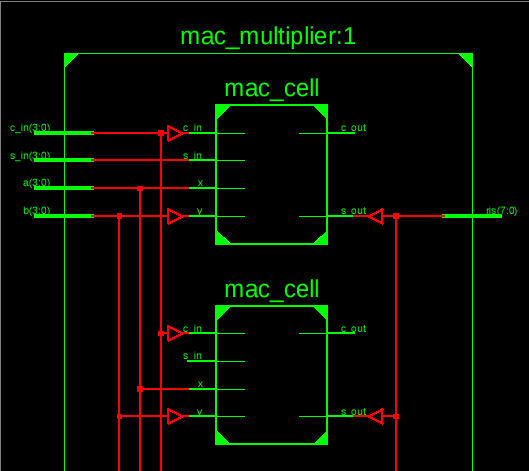
\includegraphics[scale=0.65]{esercizio13/images/mac_mul.png}
	\caption{Mac Multiplier}
\end{figure}

Viene mostrato un esempio di moltiplicatore a celle MAC 2x2 (purtroppo
lo schematico se preso nella sua interezza non rendeva visibili i
segnali), per la gestione dei segnali di interconnessione si � ricorso
all' uso di un costrutto matrix, data la simmetria del circuito in
cui vengono gestiti i vari carry e somme parziali di ingresso ed uscita,
si � scelto di instanziare prima le righe, gestendo le somme parziali
in ingresso ed in carry in uscita, alla successiva riga invece vanno
gestiti i carry in ingresso e le somme in uscita.

\begin{table}[H]
\begin{minipage}[t]{0.5\paperwidth}%
\begin{tabular}{|>{\centering}p{3cm}||c||c||c||>{\centering}p{2cm}|}
\hline 
Numero di bit operandi & Numero di slice & Numero di four LUT & Tempo di calcolo & Tempo di

calcolo per cella(stimato)\tabularnewline
\hline 
\hline 
2x2 & 4 & 8 & 8,978 ps & 1,122 ps\tabularnewline
\hline 
\hline 
4x4 & 17 & 32 & 14,557 ps & 0,7278 ps\tabularnewline
\hline 
\hline 
8x8 & 65 & 128 & 25,026 ps & 0,579 ps\tabularnewline
\hline 
\hline 
16x16 & 256 & 512 & 51,175 ps & 0,556 ps\tabularnewline
\hline 
\end{tabular}%
\end{minipage}
\end{table}

Possiamo riscontrare che il sintettizzatore, mette in ogni slice una
cella MAC, lo spazio occupato quindi per ogni raddoppio di riga e
di colonna diventa quattro volte maggiore come anche il numero di
LUT quadruplica, per il numero minimale di slice presente sulla BASYS
non � possibile sintetizzare un 32x32.

I tempi di calcolo teoricamente dovrebbero essere pari a $6(n-1)T+2T$
(dove $n$ numero o di riga o di colonna essendo il moltiplicatore
simmettrico e $T$ ritardo di una porta), se dalla formula ricaviamo
$T$ al variare di $n$ notiamo che il tempo per cella descresce,
in realt� le celle vengono messe sempre pi� vicine durate l' operazione
di place and routing, dato che il loro numero aumenta e lo spazio
diminuisce, riducendo cos� la distanza fra di esse ed il tempo di
propagazione dei segnali.

\subsubsection{Moltiplicatore di Booth}

\begin{figure}[H]
	\centering
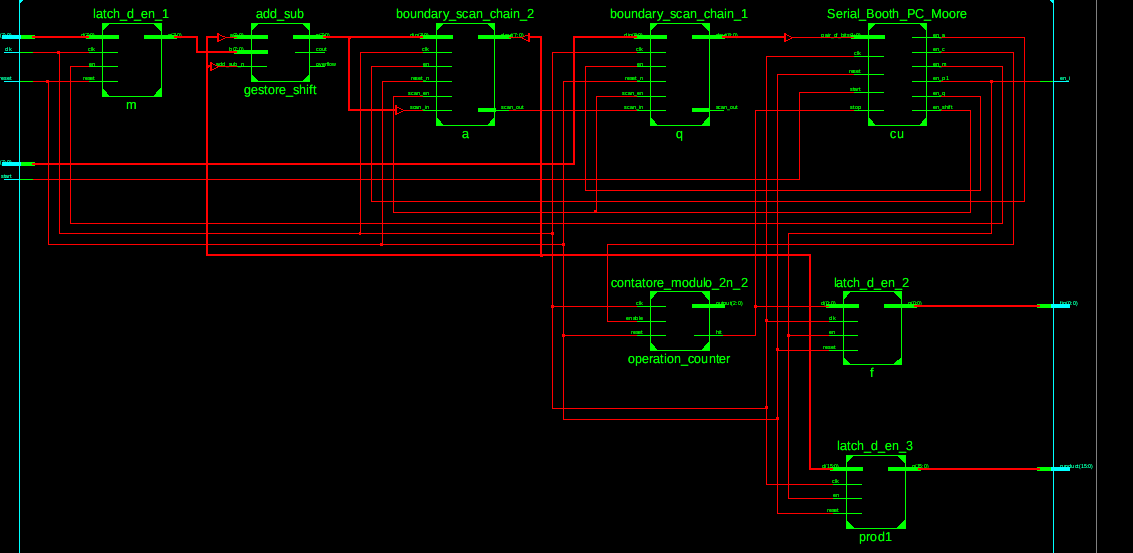
\includegraphics[scale=0.4]{esercizio13/images/Booth_mul.png}
	\caption{Booth Multiplier}
\end{figure}

\label{Booth}

Per realizzare il motiplicatore (che utilizza la codifica Booth-1),
si � utilizzato una macchina a stati finiti con i seguenti stati: 
\begin{itemize}
\item idle, stato in cui la macchina non opera; init, vi � l' inizializzazione
dei registri e delle scan chain, il moltiplicatore va salvato in un
registro, nella scan chain q il moltiplicando e a viene settata a
0; 
\item in getseq vengono letti gli ultimi due bit in uscita dalla scan chain
q, in base ai valori ne si ricava la codifica di Booth e si decide
se sommare, sottrarre prima di effettuare lo shifting o solo effettuare
quest' ultimo;
\item in inits si abilita lo shifting che verr� effettuato al passaggio
nel successivo stato shift.
\end{itemize}
La scan chain d� anche la possibilit� di essere usata come semplice
registro, difatti viene sfruttato nel caso in cui avvenga una somma
o una sottrazione, perch� prima di fare lo shiting viene caricato
il risultato di tale operazione in a e poi shiftato. La terminazione
si ha quando il contatore genera un segnale di hit, che avviene successivamente
all' ultima operazione derivante dalla codifica di Booth.

\subsection{Codice}

\noindent\begin{minipage}[t]{1\columnwidth}%
\href{run:progetti/MacMultiplier/MacMultiplier.xise}{Mac ISE}

\medskip{}

\href{run:progetti/Booth/moltiplicatore_booth.xise}{Booth ISE}%
\end{minipage}

\subsubsection{Moltiplicatore a celle Mac}

\lstinputlisting [language=VHDL,caption={Definizione della carry save cell},firstline=4] {progetti/MacMultiplier/mac_multiplier.vhd}\selectlanguage{italian}%

